% Autor: Igor Mjasojedov <xmjaso00@stud.fit.vutbr.cz>
% Autor: Alex Sporni <xsporn01@stud.fit.vutbr.cz>
% Autor: Richard Borbély <xborbe00@stud.fit.vutbr.cz>
% Autor: Daniel Weis <xweisd00@stud.fit.vutbr.cz>


\documentclass[a4paper, 11pt]{article}


\usepackage[czech]{babel}
\usepackage[utf8]{inputenc}
\usepackage[left=2cm, top=3cm, text={17cm, 24cm}]{geometry}
\usepackage{times}
\usepackage{verbatim}
\usepackage{graphicx}
\usepackage[unicode]{hyperref}
\usepackage[normalem]{ulem}
\useunder{\uline}{\ul}{}



\newcommand{\RNum}[1]{\uppercase\expandafter{\romannumeral #1\relax}}

\begin{document}

\begin{titlepage}
		\begin{center}
		\Huge
			\textsc{Vysoké učení technické v~Brně} \\
		\huge
		\textsc{Fakulta informačních technologií} \\
			
\includegraphics[width=0.77\linewidth]{logo/logo.pdf} \\

			\vspace{\stretch{0.382}}

			\Huge{Projektová dokumentácia} \\
			\LARGE{\textbf{Implementácia prekladača imperatívneho jazyka IFJ18}} \\
			\Large{Tým 78, varianta \RNum{2}}
			\vspace{\stretch{0.618}}
		\end{center}

		\begin{minipage}{0.4 \textwidth}
			{\Large \today}
		\end{minipage}
		\hfill
		\begin{minipage}[r]{0.6 \textwidth}
			\Large
			\begin{tabular}{l l l}
				\textbf{Igor Mjasojedov} & \textbf{(xmjaso00)} & \quad 25\,\% \\
				Richard Borbély & (xborbe00) & \quad 25\,\% \\				
				Alex Sporni & (xsporn01) & \quad 25\,\% \\
				Daniel Weis & (xweisd00) & \quad 25\,\% \\
			\end{tabular}
		\end{minipage}
\end{titlepage}



\pagenumbering{Roman}
\setcounter{page}{0}
\tableofcontents
\newpage

\pagenumbering{arabic}
\setcounter{page}{1}
\section{Úvod}

Cieľom projektu, bolo vytvoriť program v~jazyku C, ktorý má za úlohu načítať zdrojový kód, v~zdrojovom jazyku IFJ18, ktorý je zjednodušenou podmnožinou jazyka Ruby 2.0 a~preložiť ho do cieľového jazyka IFJcode18 (medzikód). 

Zvolili sme si zadanie II, v~ktorom bolo za úlohu implementovať tabuľku symbolov pomocou tabuľky s rozptýlenými položkami.
Výsledný program funguje ako konzolová aplikácia, ktorá načíta riadiaci program v jazyku IFJ18 zo štandardného vstupu a~bude generovať výsledný medzikód v IFJcode18 na štandardný výstup.
\section{Implementácia}

\subsection{Lexikálna analýza}
Pri tvorbe prekladača sme začali implementáciou lexikálnej analýzy. Lexikálna analýza je zostrojená implementáciou dopredu vytvoreného deterministického konečného  automatu \ref{obrazok:KA}, ktorý pozostáva z~dočasných (pomocných) a~koncových stavov. Na základe v~ktorom stave skončí, určí typ tokenu.

Hlavnou časťou lexikálnej analýzy z~ktorej vychádzame je funkcia \texttt{get\_next\_token}, ktorá spracováva vstup znak po znaku zo zdrojového súboru a~prevádza lexémy na tokeny, ktoré sú ďalej spracovávané syntaktickou analýzou. Token sa skladá z~typu a~atribútu. Srdcom funkcie \texttt{get\_next\_token} je \texttt{switch}, kde každý jeden prípad \texttt{case} je reprezentovaný práve jedným stavom KA, ktorý sa nachádza v~nekonečnom cykle. Komentáre a~biele znaky sú lexikálnym analyzátorom ignorované. Pokiaľ sa načítaný znak nezhoduje so žiadnym znakom, ktorý jazyk IFJ18 povoluje, program sa ukončí a~vráti prislúchajúcu návratovú hodnotu.

\subsection{Syntaktická analýza}
Implementácia prebiehala na základe predom vytvorenej LL--gramatiky s využitím dopočučenej metódy rekurzívneho zostupu. Ku každej sade pravidiel určitého neterminálu prislúchala určitá funkcia. Pre správne priebežné vyhodnocovanie jednotlivých pravidiel sa žiada o~ďalší token modul SCANNER pomocou makra \texttt{GET\_NEXT\_TOKEN()}, ktoré nám v~prípade chyby v~lexikálnej analýze vráti príslušnú chybovú hodnotu. Počas analýzy sa nám priebežne volajú funkcie modulu GENERATOR podľa aktuálne spracovávanej konštrukcie jazyka.

\subsubsection{Syntaktická analýza výrazov} 
Výrazy sme spracovávali s~využití precedenčnej syntaktickej analýzy. Pred samotnou implementáciou sme potrebovali vytvoriť precedenčnú tabuľku, na základe ktorej sa analýza riadila. Taktiež aj pri tejto analýze sme volali funkcie generátoru, ktorých vykonanie nám zabezpečilo korektné vytvorenie jednotlivých inštrukcií pre prácu nad zásobníkom.

\subsection{Sémantická analýza}
Všetky akcie sémantickej analýzy sa priebežne vykonávali so syntaktickou analýzou a~využívali informácie o~jednotlivých funkciách a premenných, ktoré sa priebežne uchovávali a~modifikovali v~tabuľke symbolov.Na korektné vykonanie sémantickej analýzy sme si potrebovali vytvoriť dve tabuľky symbolov, globálnu a~lokálnu. 

V~globálnej tabuľke sme uchovávali informácie o~všetkých vytvorených funkciách vrátane preddefinovaných funkií a~informácie o~premenných vytvorených v~hlavnom tele programu.

V~lokálnej tabuľke symbolov sme uchovávali informácie o~premenných vytvorených v~tele definície danej funkcie a~taktiež o~parametroch danej funkcie. Z~definície funkcie bola možnosť prístupu do globálnej tabuľky jedine k~položkám, ktoré nám reprezentovali už vytvorené funkcie a~v~prípade snahy využitia premennej, ktorej informácie boli uchované jedine v~globálnej tabuľke došlo k~sémantickej chybe, nakoľko náš jazyk nepodporoval možnosť globálnych premenných.

Najväčšou obtiaťnosťou sémantických resp. typových kontrôl sa nám zdala byť kontrola typov operandov v~definícii funkcie pri situácii kedy daný operand resp. operandy boli parametrami funkcie. Obtiaťnosť týchto kontrôl vyplývala zo samotnej konštrukcie jazyka, kde pri definícii funkcie sme nepoznali typy daných parametrov. Kvôli tejto vlastnosti jazyka sme boli nútený sémantické kontroly nad parametrami funkcie riešiť až na úrovni generovania cieľového kódu, a to spôsobom korektného generovania jednotlivých inštrukcií.


\subsection{Generovanie cieľového kódu}

Finálnou časťou celého projektu bola implementácia modulu GENERATOR, ktorý mal za úlohu generovať finálny trojadresný kód \texttt{.IFJcode18}. 
Funkcionalita modulu GENERATOR spočívala vo volaní jeho funkcií z modulov PARSER a 
PARSER\_EXPRESSIONS v priebehu syntaktickej a~sémantickej analýzy.

Generovaný kód sa priebežne zapisoval do dvoch dynamických reťazcov, ktoré nám slúžili na oddelený zápis definícii funkcii a~kódu hlavného tela programu. K~rozhodnutiu o~výbere cieľového dynamického reťazca k~zápisu aktuálne generovaného kódu nám slúžil indikátor aktuálnej pozície a~to buď tela definície funkcie alebo tela hlavného programu.

Jednotlivé funkcie tohto modulu nám zabezpečovali generovanie správnych konštrukcií kódu pri typovej kontrole výrazu, podmienenom príkaze, príkaze cyklu, pri potrebe pretypovania číselného typu, pri volaní funkcie a taktiež správnu konštrukciu definície funkcie atď\dots
\newpage
\section{Algoritmy a~dátové štruktúry}
\subsection{Tabuľka s~rozpýlenými položkami}

Tabuľku symbol sme vytvorili pomocou tabuľky s~rozptýlenými položkami, keďže sme si zvolili práve túto variantu zadania. Ako veľkosť tabuľky sme si zvolili prvočíslo 12289 z~dôvodu  percentuálne nízkej šance zhlukovania jednotlivých položiek tabuľky.    

Pri implementácii sme položku tabuľky reprezentovali štruktúrou \texttt{tHTItem}, ktorá obsahovala ukazateľ na ďalšiu položku, unikátny kľúč, ktorý nám taktiež reprezentoval názov funkcie alebo premennej. Ako poslednú súčasť štruktúry \texttt{tHTItem} sme si implementovali štruktúru \texttt{tData}, kde sme uchovávali nasledovné informácie: typ premennej/návratový typ funkcie, indikátor typu položky (funckia/premenná), indikátor overujúci predošlé definovanie funkcie, typy parametrov funkcie,  reprezentované pomocou pola znakov, v~ktorom každý jeden znak označuje typ jedného parametru.

Výber hashovacej funkcie sme uskutočnili na základe nasledujúcich nami uprednosťovaných faktorov: frekvencia kolízii, efektivita daného algoritmu a~obtiažnosť implementácie. Po porovnaní rôznych typov hash funkcií sme rozhodli pre GNU ELF Hash.

\subsection{Zásobník}

Počas syntaktickej/sémantickej analýzy výrazov v~module PARSER\_EXPRESSIONS sme bezpodmienečne potrebovali funkcionalitu zásobníku, a~preto sme museli vytvoriť aj túto dátovú štruktúru.

Základné funkcie nad štruktúrou \texttt{Item\_Stack} sme implementovali na základe nadobudnutých vedomostí z~prednášok predmetu IAL. Avšak pre potreby precedenčnej syntaktickej analýzy sme museli dodatočne implementovať špecializované funkcie vhodné na túto činnosť. 

\subsection{Dynamický reťazec}
Pri implementácii sme narazili na komplikáciu práce s reťazcami v jazyku C, a~preto sme si museli vytvoriť štruktúru \texttt{String\_DYNAMIC} a~prislúchajúce funkcie pre prácu s~ňou.

V~danej štruktúre sme uchovávali ukazateľ na reťazec, veľkosť aktuálneho reťazca a~počet bajtov pridelenej pamäte pre aktuálny reťazec. V~prípade rozširovania reťazca sme vlastnosť dynamickosti zabezpečili porovnávaním aktuálnej veľkosti reťazca a~počtu bajtov už pridelenej pamäte, kde sme v~prípade nedostatočného množstva voľnej pridelenej pamäte pristúpili k~jej rozšíreniu. 

\section{Práca v~týme}

\subsection{Príprava, plán a~spôsob práce}

Keďže sme si uvedomovali náročnosť a~rozsiahlosť daného projektu, rozhodli sme sa začať čo najskôr. Prvotná príprava a~plány započali na úvodných prednáškach predmetu IFJ a~IAL. Prácu sme si delili postupne a~rovnomerne, keďže sme zo začiatku nemali jasnú predstavu finálneho konceptu a~implementácie, neskôr sme si jednotlivé časti rozdelili podľa schopností jednotlivca.

\subsection{Komunikácia}

Komunikácia prebiehala najmä osobne, zo začiatku sme sa dohodli na pravidelných stretnutiach vo~fakultnej knižnici, menšie pripomienky a~otázky sme diskutovali pomocou sociálnych sietí.

\subsection{Verzovací systém}

Pre správu verzií súborov projektu sme používali verzovací systém Git. Hlavným dôvodom bola kompatibilita s~vývojovým prostredím CLion. Ako vzdialený repozitár nám poslúžil GitHub, ktorý nám ponúkol okrem privátneho repozitára možnosť sledovať prácu jednotlivca a~graf priebežného vývoja. Väčšinu práce na jednotlivých častiach projektu sme riešili na oddelených vetvách aby sa zamedzidlo prípadným konfliktom pri správe aktuálnych verzií. Po schválení vedúcim týmu sme jednotlivé vetvy zlúčili do hlavnej vývojovej vetvy.

\subsection{Prekladový systém}
Preklad nášho projektu sme zabezpečovali pomocou nástroja CMake alebo GNU Make.

\subsubsection{GNU Make}
V zadaní sme mali špecifikovanú požiadavku na pridanie súboru \texttt{Makefile} do odovzdávaného archívu, na základe ktorej sme museli zabezpečiť funkcionalitu prekladu aj cez tento nástroj.

Nami vytvorený súbor \texttt{Makefile} disponoval nielen základnou funkcionalitou prekladu zdrojových\linebreak súborov -- \texttt{make}, ale aj doplňujúcimi príkazmy na vytvorenie \texttt{.zip} archívu -- \texttt{make\,zip},\linebreak
vytvorenie \texttt{tar.gz} archívu -- \texttt{make\,pack} a~taktiež na vymazanie prekladom vytvorených objektových\linebreak a binárnych súborov -- \texttt{make\,clean}.

\subsubsection{CMake}

Nakoľko sme celý projekt vyvájali hlavne vo vývojovom prostredí CLion, ktorý má už v sebe štandardne zabudovaný nástroj CMake, sa nám zjednodušila práca s prekladom celého projektu nakoľko sa všetky novo pridané súbory automaticky pridali do súboru \texttt{CMakeLists.txt}, kde boli taktiež nastavené všetky pravidlá pre preklad.

\subsection{Rozdelenie práce}
Prácu na projekte sme si rozdelili rovným dielom, Náplň práce jednotlivých členov je popísana v tabuľke \ref{tabulka:rozdelenie_prace}
\bigskip
\begin{table}[!ht]
\begin{tabular}{|l|l|}
\hline
Člen týmu                & \multicolumn{1}{c|}{Pridelená práca}   \\ \hline
\textbf{Igor Mjasojedov} & \begin{tabular}[c]{@{}l@{}}Implementácia syntaktickej analýzy a sémantickej analýzy (modul parser), \\ revízia kódu, vedenie týmu, organizácia práce, štruktúa projektu\end{tabular} \\ \hline
Alex Sporni              & \begin{tabular}[c]{@{}l@{}}Implementácia lexikálnej analýzy (modul scanner), vytvorenie dokumentácie,\\ vytvorenie prezentácie\end{tabular}                                          \\ \hline
Richard Borbély          & Generovanie cieľového kódu, testovanie                                                                                                                                               \\ \hline
Daniel Weis              & \begin{tabular}[c]{@{}l@{}}Implementácia dátových štruktúr (tabuľka s rozptýlenými položkami), \\ zásobník, testovanie\end{tabular}                                                  \\ \hline
\end{tabular}
\caption{Rozdelenie práce v~týme}
\label{tabulka:rozdelenie_prace}
\end{table}
\section{Záver}

K~riešeniu projektu sme pristupovali zodpovedne a~systematicky, samotný rozsah projektu a~náročnosť boli pre nás výzvou, s~akou sme sa na iných predmetoch doposial nestretli. Projekt nám okrem mnohých praktických znalostí, pomohol zlepšiť komunikáciu v~rámci skupiny a~lepšie formulovať myšlienky pri pripomienkach. 

Pri implementácii sme sa stretli s~komplikáciami ohladne typovej kontroly pri behu programu. Nejasnosti, ktoré vyplývali zo zadania sme riešili na diskusnom fóre určenom pre projekt, kde sa daná problematika väčšinou už rozoberala.
Správnosť našich riešení sme si pravidelne overovali pomocou automatických testov, ktoré sme si vytvorili a~taktiež pokusnými odovzdaniami, ktoré nám pomohli odhaliť nedostatky jednotlivých modulov projektu.
\newpage
\section{Pouzitá literatúra}
\newpage
\section{Príloha}
\appendix

\section{LL Gramatika}
\begin{table}[!ht]
\centering
\begin{tabular}{lllll}
\textless{}program\textgreater{}        &  &  & $\rightarrow$ & EOF                                                                                                                              \\
                                        &  &  & $\rightarrow$ & EOL \textless{}program\textgreater{}                                                                                             \\
                                        &  &  & $\rightarrow$ & def \textless{}def\textgreater{} EOL \textless{}program\textgreater{}                                                              \\
                                        &  &  & $\rightarrow$ & \textless{}statement\textgreater{} EOL \textless{}program\textgreater{}                                                            \\
\textless{}def\textgreater{}            &  &  & $\rightarrow$ & id (\textless{}param\_list\textgreater{}) EOL \textless{}state\_list\textgreater{} end                                             \\
\textless{}state\_list\textgreater{}    &  &  & $\rightarrow$ & \textless{}statement\textgreater{} EOL \textless{}state\_list\textgreater{}                                                        \\
                                        &  &  & $\rightarrow$ & $\varepsilon$                                                                                                                    \\
                                        &  &  & $\rightarrow$ & EOL \textless{}state\_list\textgreater{}                                                                                         \\
\textless{}statement\textgreater{}      &  &  & $\rightarrow$ & if \textless{}expression\textgreater then EOL \textless{}state\_list\textgreater{} else EOL \textless{}state\_list\textgreater{} end \\
                                        &  &  & $\rightarrow$ & while \textless{}expression\textgreater{} do EOL \textless{}state\_list\textgreater{} end                                            \\
                                        &  &  & $\rightarrow$ & id = \textless{}id\_assign\textgreater{}                                                                                         \\
                                        &  &  & $\rightarrow$ & \textless{}fnc\_call\textgreater{}                                                                                               \\
                                        &  &  & $\rightarrow$ & \textless{}expression\textgreater{}                                                                                              \\
\textless{}id\_assign\textgreater{}     &  &  & $\rightarrow$ & \textless{}fnc\_call\textgreater{}                                                                                               \\
                                        &  &  & $\rightarrow$ & \textless{}expression\textgreater{}                                                                                              \\
\textless{}param\_list\textgreater{}    &  &  & $\rightarrow$ & id \textless{}param\_next\textgreater{}                                                                                          \\
                                        &  &  & $\rightarrow$ & $\varepsilon$                                                                                                                    \\
\textless{}param\_next\textgreater{}    &  &  & $\rightarrow$ & , id \textless{}param\_next\textgreater{}                                                                                        \\
                                        &  &  & $\rightarrow$ & $\varepsilon$                                                                                                                    \\
\textless{}fnc\_call\textgreater{}      &  &  & $\rightarrow$ & id \textless{}argument\_list\textgreater{}                                                                                       \\
                                        &  &  & $\rightarrow$ & inputs \textless{}argument\_list\textgreater{}                                                                                   \\
                                        &  &  & $\rightarrow$ & inputf \textless{}argument\_list\textgreater{}                                                                                   \\
                                        &  &  & $\rightarrow$ & inputi \textless{}argument\_list\textgreater{}                                                                                   \\
                                        &  &  & $\rightarrow$ & print \textless{}argument\_list\textgreater{}                                                                                    \\
                                        &  &  & $\rightarrow$ & length \textless{}argument\_list\textgreater{}                                                                                   \\
                                        &  &  & $\rightarrow$ & substr \textless{}argument\_list\textgreater{}                                                                                   \\
                                        &  &  & $\rightarrow$ & ord \textless{}argument\_list\textgreater{}                                                                                      \\
                                        &  &  & $\rightarrow$ & chr \textless{}argument\_list\textgreater{}                                                                                      \\
\textless{}argument\_list\textgreater{} &  &  & $\rightarrow$ & (\textless{}arguments\textgreater{})                                                                                             \\
                                        &  &  & $\rightarrow$ & \textless{}arguments\textgreater{}                                                                                               \\
\textless{}arguments\textgreater{}      &  &  & $\rightarrow$ & \textless{}term\textgreater{} \textless{}argument\_next\textgreater{}                                                              \\
                                        &  &  & $\rightarrow$ & $\varepsilon$                                                                                                                    \\
\textless{}argument\_next\textgreater{} &  &  & $\rightarrow$ & , \textless{}term\textgreater{} \textless{}argument\_next\textgreater{}                                                            \\
                                        &  &  & $\rightarrow$ & $\varepsilon$                                                                                                                    \\
\textless{}term\textgreater{}           &  &  & $\rightarrow$ & id                                                                                                                               \\
                                        &  &  & $\rightarrow$ & INTEGER\_VALUE                                                                                                                   \\
                                        &  &  & $\rightarrow$ & FLOAT\_VALUE                                                                                                                     \\
                                        &  &  & $\rightarrow$ & STRING\_VALUE                                                                                                                   
\end{tabular}
\caption{LL -- gramatika riadiaca syntaktickú analýzu}
\label{tabulka:LL_gram}
\end{table}

\newpage
\section{Precedenčná tabuľka}
\begin{table}[!ht]
\centering
\begin{tabular}{|l|c|c|c|c|c|c|c|c|l|l|l|l|l|l|}
\hline
                        & \multicolumn{1}{l|}{\textbf{+}}              & \multicolumn{1}{l|}{\textbf{-}}              & \multicolumn{1}{l|}{\textbf{*}}              & \multicolumn{1}{l|}{\textbf{/}}              & \multicolumn{1}{l|}{\textbf{\textless{}}}    & \multicolumn{1}{l|}{\textbf{$\leq$}}         & \multicolumn{1}{l|}{\textbf{\textgreater{}}} & \multicolumn{1}{l|}{\textbf{$\geq$}}         & \textbf{==}             & \textbf{!=}             & \textbf{(}           & \textbf{)}              & \textbf{ID}          & \textbf{\$}             \\ \hline
\textbf{+}              & \textgreater{}                               & \textgreater{}                               & \textless{}                                  & \textless{}                                  & \textgreater{}                               & \textgreater{}                               & \textgreater{}                               & \textgreater{}                               & \textgreater{}          & \textgreater{}          & \textless{}          & \textgreater{}          & \textless{}          & \textgreater{}          \\ \hline
\textbf{-}              & \textgreater{}                               & \textgreater{}                               & \textless{}                                  & \textless{}                                  & \textgreater{}                               & \textgreater{}                               & \textgreater{}                               & \textgreater{}                               & \textgreater{}          & \textgreater{}          & \textless{}          & \textgreater{}          & \textless{}          & \textgreater{}          \\ \hline
\textbf{*}              & \textgreater{}                               & \textgreater{}                               & \textgreater{}                               & \textgreater{}                               & \textgreater{}                               & \textgreater{}                               & \textgreater{}                               & \textgreater{}                               & \textgreater{}          & \textgreater{}          & \textless{}          & \textgreater{}          & \textless{}          & \textgreater{}          \\ \hline
\textbf{/}              & \textgreater{}                               & \textgreater{}                               & \textgreater{}                               & \textgreater{}                               & \textgreater{}                               & \textgreater{}                               & \textgreater{}                               & \textgreater{}                               & \textgreater{}          & \textgreater{}          & \textless{}          & \textgreater{}          & \textless{}          & \textgreater{}          \\ \hline
\textbf{\textless{}}    & \textless{}                                  & \textless{}                                  & \textless{}                                  & \textless{}                                  &                                              &                                              &                                              &                                              & \textgreater{}          & \textgreater{}          & \textless{}          & \textgreater{}          & \textless{}          & \textgreater{}          \\ \hline
\textbf{$\leq$}         & \textless{}                                  & \textless{}                                  & \textless{}                                  & \textless{}                                  &                                              &                                              &                                              &                                              & \textgreater{}          & \textgreater{}          & \textless{}          & \textgreater{}          & \textless{}          & \textgreater{}          \\ \hline
\textbf{\textgreater{}} & \textless{}                                  & \textless{}                                  & \textless{}                                  & \textless{}                                  &                                              &                                              &                                              &                                              & \textgreater{}          & \textgreater{}          & \textless{}          & \textgreater{}          & \textless{}          & \textgreater{}          \\ \hline
\textbf{$\geq$}         & \textless{}                                  & \textless{}                                  & \textless{}                                  & \textless{}                                  &                                              &                                              &                                              &                                              & \textgreater{}          & \textgreater{}          & \textless{}          & \textgreater{}          & \textless{}          & \textgreater{}          \\ \hline
\textbf{==}             & \multicolumn{1}{l|}{\textless{}}             & \multicolumn{1}{l|}{\textless{}}             & \multicolumn{1}{l|}{\textless{}}             & \multicolumn{1}{l|}{\textless{}}             & \multicolumn{1}{l|}{\textless{}}             & \multicolumn{1}{l|}{\textless{}}             & \multicolumn{1}{l|}{\textless{}}             & \multicolumn{1}{l|}{\textless{}}             &                         &                         & \textless{}          & \textgreater{}          & \textless{}          & \textgreater{}          \\ \hline
\textbf{!=}             & \multicolumn{1}{l|}{\textless{}}             & \multicolumn{1}{l|}{\textless{}}             & \multicolumn{1}{l|}{\textless{}}             & \multicolumn{1}{l|}{\textless{}}             & \multicolumn{1}{l|}{\textless{}}             & \multicolumn{1}{l|}{\textless{}}             & \multicolumn{1}{l|}{\textless{}}             & \multicolumn{1}{l|}{\textless{}}             &                         &                         & \textless{}          & \textgreater{}          & \textless{}          & \textgreater{}          \\ \hline
\textbf{(}              & \multicolumn{1}{l|}{\textless{}}             & \multicolumn{1}{l|}{\textless{}}             & \multicolumn{1}{l|}{\textless{}}             & \multicolumn{1}{l|}{\textless{}}             & \multicolumn{1}{l|}{\textless{}}             & \multicolumn{1}{l|}{\textless{}}             & \multicolumn{1}{l|}{\textless{}}             & \multicolumn{1}{l|}{\textless{}}             & \textless{}             & \textless{}             & \textless{}          & =                       & \textless{}          &                         \\ \hline
\textbf{)}              & \multicolumn{1}{l|}{\textbf{\textgreater{}}} & \multicolumn{1}{l|}{\textbf{\textgreater{}}} & \multicolumn{1}{l|}{\textbf{\textgreater{}}} & \multicolumn{1}{l|}{\textbf{\textgreater{}}} & \multicolumn{1}{l|}{\textbf{\textgreater{}}} & \multicolumn{1}{l|}{\textbf{\textgreater{}}} & \multicolumn{1}{l|}{\textbf{\textgreater{}}} & \multicolumn{1}{l|}{\textbf{\textgreater{}}} & \textbf{\textgreater{}} & \textbf{\textgreater{}} & \textbf{}            & \textbf{\textgreater{}} & \textbf{}            & \textbf{\textgreater{}} \\ \hline
\textbf{ID}             & \multicolumn{1}{l|}{\textbf{\textgreater{}}} & \multicolumn{1}{l|}{\textbf{\textgreater{}}} & \multicolumn{1}{l|}{\textbf{\textgreater{}}} & \multicolumn{1}{l|}{\textbf{\textgreater{}}} & \multicolumn{1}{l|}{\textbf{\textgreater{}}} & \multicolumn{1}{l|}{\textbf{\textgreater{}}} & \multicolumn{1}{l|}{\textbf{\textgreater{}}} & \multicolumn{1}{l|}{\textbf{\textgreater{}}} & \textbf{\textgreater{}} & \textbf{\textgreater{}} & \textbf{}            & \textbf{\textgreater{}} & \textbf{}            & \textbf{\textgreater{}} \\ \hline
\textbf{\$}             & \multicolumn{1}{l|}{\textbf{\textless{}}}    & \multicolumn{1}{l|}{\textbf{\textless{}}}    & \multicolumn{1}{l|}{\textbf{\textless{}}}    & \multicolumn{1}{l|}{\textbf{\textless{}}}    & \multicolumn{1}{l|}{\textbf{\textless{}}}    & \multicolumn{1}{l|}{\textbf{\textless{}}}    & \multicolumn{1}{l|}{\textbf{\textless{}}}    & \multicolumn{1}{l|}{\textbf{\textless{}}}    & \textbf{\textless{}}    & \textbf{\textless{}}    & \textbf{\textless{}} & \textbf{}               & \textbf{\textless{}} & \textbf{}               \\ \hline
\end{tabular}
\caption{Precedenčná tabuľka použitá pri precedenčnej syntaktickej analýze výrazov}
\end{table}

\newpage
\section{Diagram konečného automatu pre lexikálny analyzátor}
\begin{figure}[!ht]
\centering
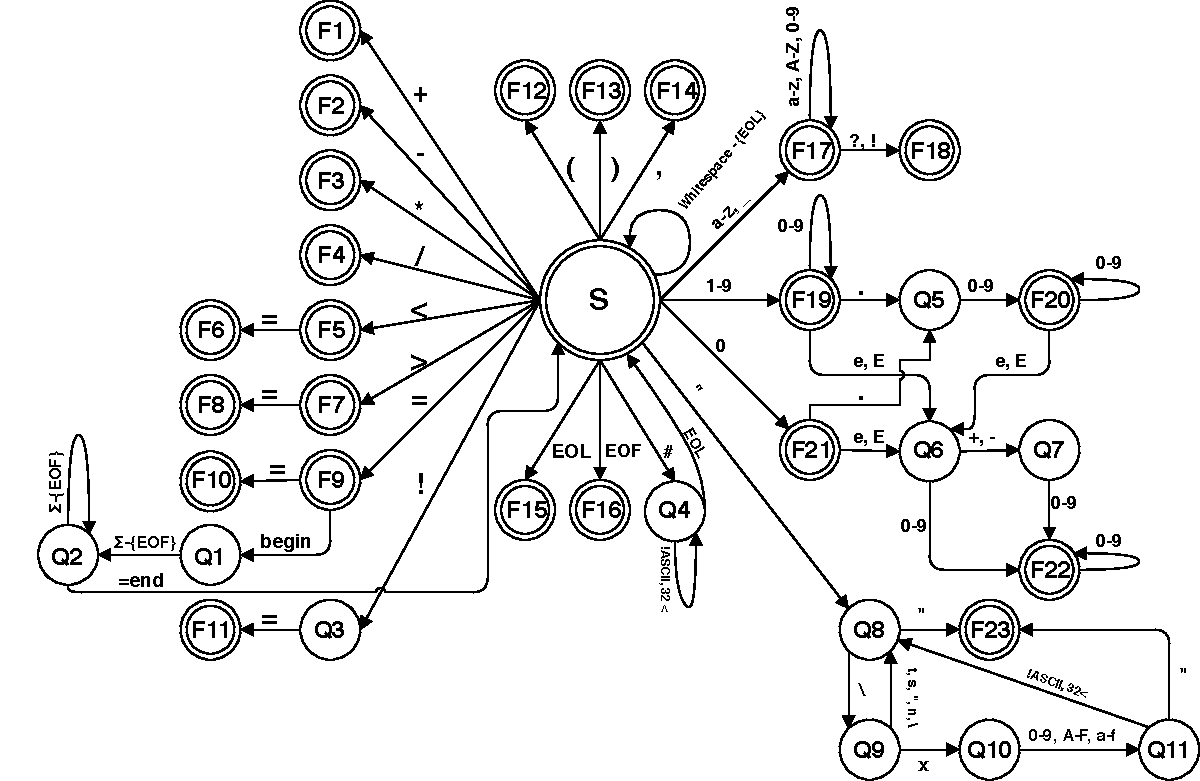
\includegraphics[width=1.0\linewidth]{automata/automata.pdf}
\caption{Diagram konečného automatu pre lexikálny analyzátor}
\label{obrazok:KA}
\end{figure}
\bigskip
\Large
\textbf{Legenda:}
\begin{table}[!ht]
\begin{tabular}{llllllll}
\textbf{S}   & START            & \textbf{F12} & LEFT\_BRACKET           &   \textbf{Q1}  & BLOCK\_COMMENTARY      \\
\textbf{F1}  & PLUS             & \textbf{F13} & RIGHT\_BRACKET          &   \textbf{Q2}  & COMMENT\_IGNORE        \\
\textbf{F2}  & MINUS            & \textbf{F14} & COMMA                   &   \textbf{Q3}  & NOT                    \\
\textbf{F3}  & MUL              & \textbf{F15} & EOL                     &   \textbf{Q4}  & LINE\_COMMENTARY       \\
\textbf{F4}  & DIV              & \textbf{F16} & EOF                     &   \textbf{Q5}  & FLOATING\_NUMBER       \\
\textbf{F5}  & LESS             & \textbf{F17} & ID\_KEY                 &   \textbf{Q6}  & E\_NUMBER              \\
\textbf{F6}  & LESS\_EQUAL      & \textbf{F18} & FUNCTION\_ID            &   \textbf{Q7}  & PLUS\_MINUS            \\
\textbf{F7}  & GREATER          & \textbf{F19} & INTEGER\_NUMBER         &   \textbf{Q8}  & STRING                 \\
\textbf{F8}  & GREATER\_EQUAL   & \textbf{F20} & FINAL\_FLOAT\_NUMBER\_1 &   \textbf{Q9}  & STRING\_ESCAPE         \\
\textbf{F9}  & ASSIGN           & \textbf{F21} & ZERO\_NUMBER            &   \textbf{Q10} & STRING\_HEXA           \\
\textbf{F10} & EQUAL            & \textbf{F22} & FINAL\_FLOAT\_NUMBER\_2 &   \textbf{Q11} & STRING\_HEXA\_ADVANCED \\
\textbf{F11} & NOT EQUAL        & \textbf{F23} & STRING\_F               &                &                       
\end{tabular}
\end{table}

\section{LL -- tabulka}
\begin{table}[ht]
\centering
%\includegraphics[scale = 1.02]{}
\caption{LL -- tabuľka}
\end{table}


\end{document}
